\documentclass{standalone}
\usepackage{amsmath}
\usepackage[dvipsnames]{xcolor}
\usepackage{tikz} 
\usetikzlibrary{arrows, decorations.markings,decorations.pathreplacing,angles,quotes}
\usepackage{microtype}
\usepackage{fourier}

\definecolor{py_blue}{rgb}{0.12156862745098039, 0.4666666666666667, 0.7058823529411765}
\definecolor{py_orange}{rgb}{1.0, 0.4980392156862745, 0.054901960784313725}
\definecolor{py_green}{rgb}{0.17254901960784313, 0.6274509803921569, 0.17254901960784313}
\definecolor{py_red}{rgb}{0.8392156862745098, 0.15294117647058825, 0.1568627450980392}
\definecolor{py_purple}{rgb}{0.5803921568627451, 0.403921568627451, 0.7411764705882353}

\begin{document}

\begin{tikzpicture}
	\node[anchor=south west,inner sep=0] (Bild) at (0,0) {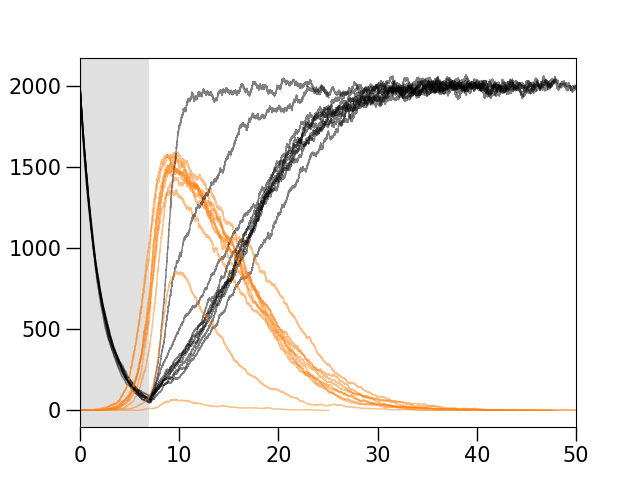
\includegraphics[scale=0.39]{trajectories_blank}};
   		\begin{scope}[x=(Bild.south east),y=(Bild.north west)]
   			        	
        	\node at ([yshift=-.2cm]Bild.south) {time [days]};
        	\node[rotate=90] at ([xshift=-.15cm]Bild.west) {population size};

        			
			\node[rotate=90,opacity=.5] at ([xshift=-1.9cm,yshift=1.cm]Bild.center) {\scriptsize treatment};   
			\node[rotate=90,opacity=.5] at ([xshift=-2.1cm,yshift=1.cm]Bild.center) {\scriptsize antibiotic}; 
			
			\draw[thick, color = black] ([yshift=.5cm,xshift=.75cm]Bild.center) -- node[right=4pt] {\small sensitive} ([xshift=1cm,yshift=.5cm]Bild.center);
			\draw[thick, color = py_orange] ([yshift=0.1cm,xshift=.75cm]Bild.center) -- node[right=4pt] {\color{black}\small resistant} ([xshift=1cm,yshift=0.1cm]Bild.center);
 			
    	\end{scope}
\end{tikzpicture}

\end{document}